% Required packages: pgfplots, lmodern
% Required TikZ libraries: none
% Target width: 160 mm maximum
% Minimum text size: 9 pt
% Colour/greyscale intent: colour_and_greyscale, direct labels and line styles
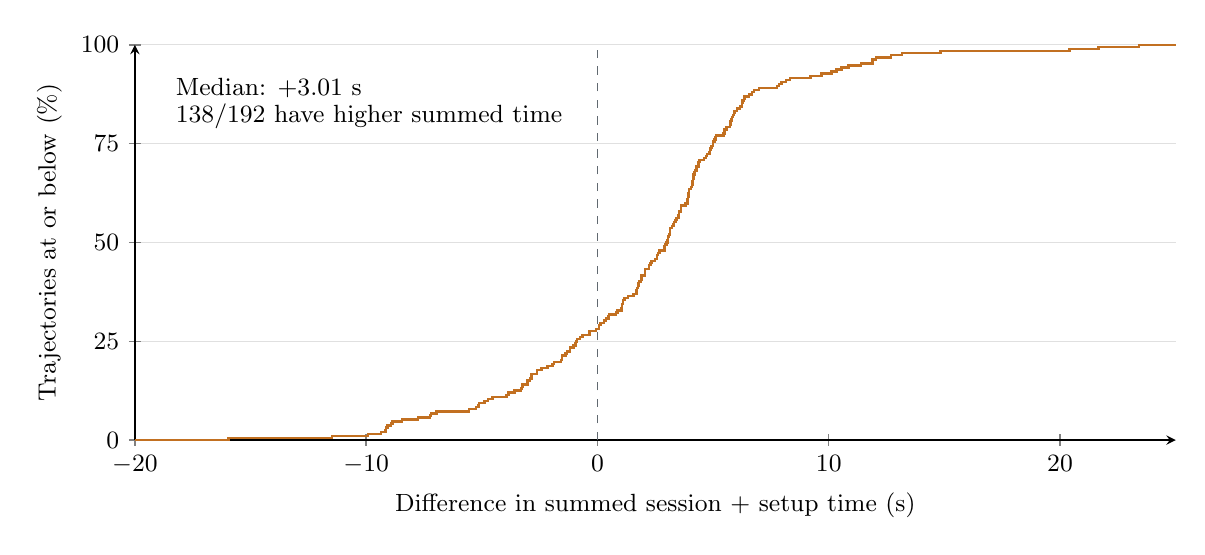
\begin{tikzpicture}
\definecolor{ealblue}{HTML}{165D81}
\definecolor{ordinaryorange}{HTML}{C27021}
\definecolor{neutralgrey}{HTML}{616970}
\pgfplotsset{compat=1.18,
  every axis/.append style={
    width=148mm,height=66mm,
    font=\fontsize{9}{11}\selectfont,
    tick label style={font=\fontsize{9}{11}\selectfont},
    label style={font=\fontsize{9}{11}\selectfont},
    title style={font=\fontsize{10}{12}\selectfont},
    legend style={font=\fontsize{9}{11}\selectfont,draw=none,fill=none},
    axis lines=left,axis line style={line width=0.5pt},
    tick style={line width=0.5pt},
    grid style={line width=0.4pt,black!12},
    scaled ticks=false,clip=false}}
\begin{axis}[xmin=-20,xmax=25,ymin=0,ymax=100,xtick={-20,-10,0,10,20},ytick={0,25,50,75,100},xlabel={Difference in summed session + setup time (s)},ylabel={Trajectories at or below (\%)},ymajorgrids=true]
\addplot[neutralgrey,dashed,line width=0.5pt,no marks] coordinates {(0,0) (0,100)};
\addplot[ordinaryorange,line width=0.9pt,no marks,const plot] coordinates {(-20,0) (-15.94272586,0.5208333333) (-11.48390383,1.041666667) (-9.932111153,1.5625) (-9.365241563,2.083333333) (-9.170126744,2.604166667) (-9.133382076,3.125) (-9.067906908,3.645833333) (-8.932867727,4.166666667) (-8.868196331,4.6875) (-8.448241529,5.208333333) (-7.761638205,5.729166667) (-7.231470037,6.25) (-7.205101627,6.770833333) (-6.952903846,7.291666667) (-5.557344284,7.8125) (-5.259894141,8.333333333) (-5.148155175,8.854166667) (-5.116078168,9.375) (-4.892470915,9.895833333) (-4.739298292,10.41666667) (-4.53540559,10.9375) (-3.933080573,11.45833333) (-3.846525598,11.97916667) (-3.594064904,12.5) (-3.307158952,13.02083333) (-3.270402303,13.54166667) (-3.250407929,14.0625) (-3.034977795,14.58333333) (-3.015354455,15.10416667) (-2.909942854,15.625) (-2.859519142,16.14583333) (-2.854230646,16.66666667) (-2.623002243,17.1875) (-2.609195684,17.70833333) (-2.42226147,18.22916667) (-2.163701613,18.75) (-1.949000744,19.27083333) (-1.879606107,19.79166667) (-1.573349319,20.3125) (-1.544513148,20.83333333) (-1.542789149,21.35416667) (-1.382855518,21.875) (-1.312543858,22.39583333) (-1.190420943,22.91666667) (-1.185035184,23.4375) (-1.026182857,23.95833333) (-0.95468713,24.47916667) (-0.917661715,25) (-0.877525533,25.52083333) (-0.760917581,26.04166667) (-0.646392037,26.5625) (-0.345442532,27.08333333) (-0.33570327,27.60416667) (-0.06335573,28.125) (0.068466275,28.64583333) (0.075732349,29.16666667) (0.131050104,29.6875) (0.290083635,30.20833333) (0.377039366,30.72916667) (0.4718182,31.25) (0.502267194,31.77083333) (0.793227413,32.29166667) (0.86123415,32.8125) (1.032325238,33.33333333) (1.057636053,33.85416667) (1.058943187,34.375) (1.093335337,34.89583333) (1.1039367,35.41666667) (1.1608373,35.9375) (1.313938288,36.45833333) (1.556525325,36.97916667) (1.693360746,37.5) (1.694824291,38.02083333) (1.712627485,38.54166667) (1.750618472,39.0625) (1.763497908,39.58333333) (1.800895549,40.10416667) (1.879559221,40.625) (1.893191449,41.14583333) (1.896307104,41.66666667) (2.044466445,42.1875) (2.046908021,42.70833333) (2.051869019,43.22916667) (2.220513374,43.75) (2.223348985,44.27083333) (2.282870861,44.79166667) (2.337698772,45.3125) (2.490527287,45.83333333) (2.57759099,46.35416667) (2.579930953,46.875) (2.606456488,47.39583333) (2.671242594,47.91666667) (2.897239366,48.4375) (2.90370482,48.95833333) (2.916551517,49.47916667) (2.985069437,50) (3.036349952,50.52083333) (3.043797281,51.04166667) (3.044567545,51.5625) (3.097758515,52.08333333) (3.127383364,52.60416667) (3.13090609,53.125) (3.142739855,53.64583333) (3.213211294,54.16666667) (3.280008709,54.6875) (3.311217677,55.20833333) (3.363960936,55.72916667) (3.414917005,56.25) (3.50514843,56.77083333) (3.52490521,57.29166667) (3.531721781,57.8125) (3.601485953,58.33333333) (3.604167627,58.85416667) (3.621839159,59.375) (3.80231422,59.89583333) (3.882535062,60.41666667) (3.901274282,60.9375) (3.915675499,61.45833333) (3.925607451,61.97916667) (3.936240358,62.5) (3.947861706,63.02083333) (3.957719612,63.54166667) (4.038094831,64.0625) (4.089681934,64.58333333) (4.100624567,65.10416667) (4.110382908,65.625) (4.125228423,66.14583333) (4.146321847,66.66666667) (4.147215549,67.1875) (4.189875211,67.70833333) (4.210404886,68.22916667) (4.274778401,68.75) (4.285328397,69.27083333) (4.359206068,69.79166667) (4.366682596,70.3125) (4.420405028,70.83333333) (4.609919938,71.35416667) (4.691874769,71.875) (4.738910607,72.39583333) (4.850203565,72.91666667) (4.875890855,73.4375) (4.876396815,73.95833333) (4.927154781,74.47916667) (4.984463616,75) (4.986862961,75.52083333) (5.055457256,76.04166667) (5.095334968,76.5625) (5.129511189,77.08333333) (5.448690078,77.60416667) (5.490251956,78.125) (5.490270877,78.64583333) (5.580315455,79.16666667) (5.724769313,79.6875) (5.747234013,80.20833333) (5.747249396,80.72916667) (5.804833537,81.25) (5.814249869,81.77083333) (5.854624442,82.29166667) (5.901342715,82.8125) (5.920199708,83.33333333) (6.030446082,83.85416667) (6.168986069,84.375) (6.257343742,84.89583333) (6.257474585,85.41666667) (6.278978397,85.9375) (6.329948445,86.45833333) (6.35188986,86.97916667) (6.552886857,87.5) (6.690627101,88.02083333) (6.758918079,88.54166667) (6.990713101,89.0625) (7.769877705,89.58333333) (7.851632518,90.10416667) (7.951545512,90.625) (8.153306981,91.14583333) (8.333064133,91.66666667) (9.208129044,92.1875) (9.680892035,92.70833333) (10.11459188,93.22916667) (10.34041111,93.75) (10.55780324,94.27083333) (10.84390623,94.79166667) (11.39089786,95.3125) (11.89107135,95.83333333) (11.89748402,96.35416667) (12.05030462,96.875) (12.69917293,97.39583333) (13.1590717,97.91666667) (14.82507364,98.4375) (20.41796987,98.95833333) (21.66339772,99.47916667) (23.40844448,100) (25,100)};
\node[anchor=west,font=\fontsize{9}{11}\selectfont] at (rel axis cs:0.03,0.89) {Median: +3.01 s};
\node[anchor=west,font=\fontsize{9}{11}\selectfont] at (rel axis cs:0.03,0.82) {138/192 have higher summed time};
\end{axis}
\end{tikzpicture}
